% Created 2020-01-30 Thu 15:43
% Intended LaTeX compiler: pdflatex
\documentclass[presentation]{beamer}
\usepackage[utf8]{inputenc}
\usepackage[T1]{fontenc}
\usepackage{graphicx}
\usepackage{grffile}
\usepackage{longtable}
\usepackage{wrapfig}
\usepackage{rotating}
\usepackage[normalem]{ulem}
\usepackage{amsmath}
\usepackage{textcomp}
\usepackage{amssymb}
\usepackage{capt-of}
\usepackage{hyperref}
\usetheme{UoB}
\author{Mark Blyth}
\date{\textit{[2020-01-31 Fri]}}
\title{Homoclinics and continuations}
\hypersetup{
 pdfauthor={Mark Blyth},
 pdftitle={Homoclinics and continuations},
 pdfkeywords={},
 pdfsubject={},
 pdfcreator={Emacs 26.3 (Org mode 9.1.9)}, 
 pdflang={English}}
\begin{document}

\maketitle

\section{Background}
\label{sec:orgfb3687c}
\begin{frame}[label={sec:orgcc056ab}]{Week's goal}
\begin{itemize}
\item Reproduce some of the bifurcation diagrams from the literature
\begin{itemize}
\item Use different continuation software packages, and add them to the comparison paper once I know them well enough to do so
\end{itemize}
\item Learn how to find homoclinic bifurcations
\item Use the bifurcation tools to learn more about Krassy's cubic Lienard model
\end{itemize}
\end{frame}
\begin{frame}[label={sec:org169a6ba}]{Week's activities (week 1)}
\begin{itemize}[<+->]
\item Tried the numerical continuation of homoclinic bifurcations in the HR model, with no success
\item Followed some homoclinic bifurcations tutorials, with success
\item Tried the numerical continuation of homoclinic bifurcations in the HR model again, with no success (again)
\item Looked a bit into the maths and numerics of homoclinic bifurcations and continuation
\end{itemize}
\end{frame}


\section{Homoclinics}
\label{sec:orgbbe1357}
\begin{frame}[label={sec:org81e3b7b}]{Motivating problem}
\begin{columns}
\begin{column}{0.6\columnwidth}
\begin{center}
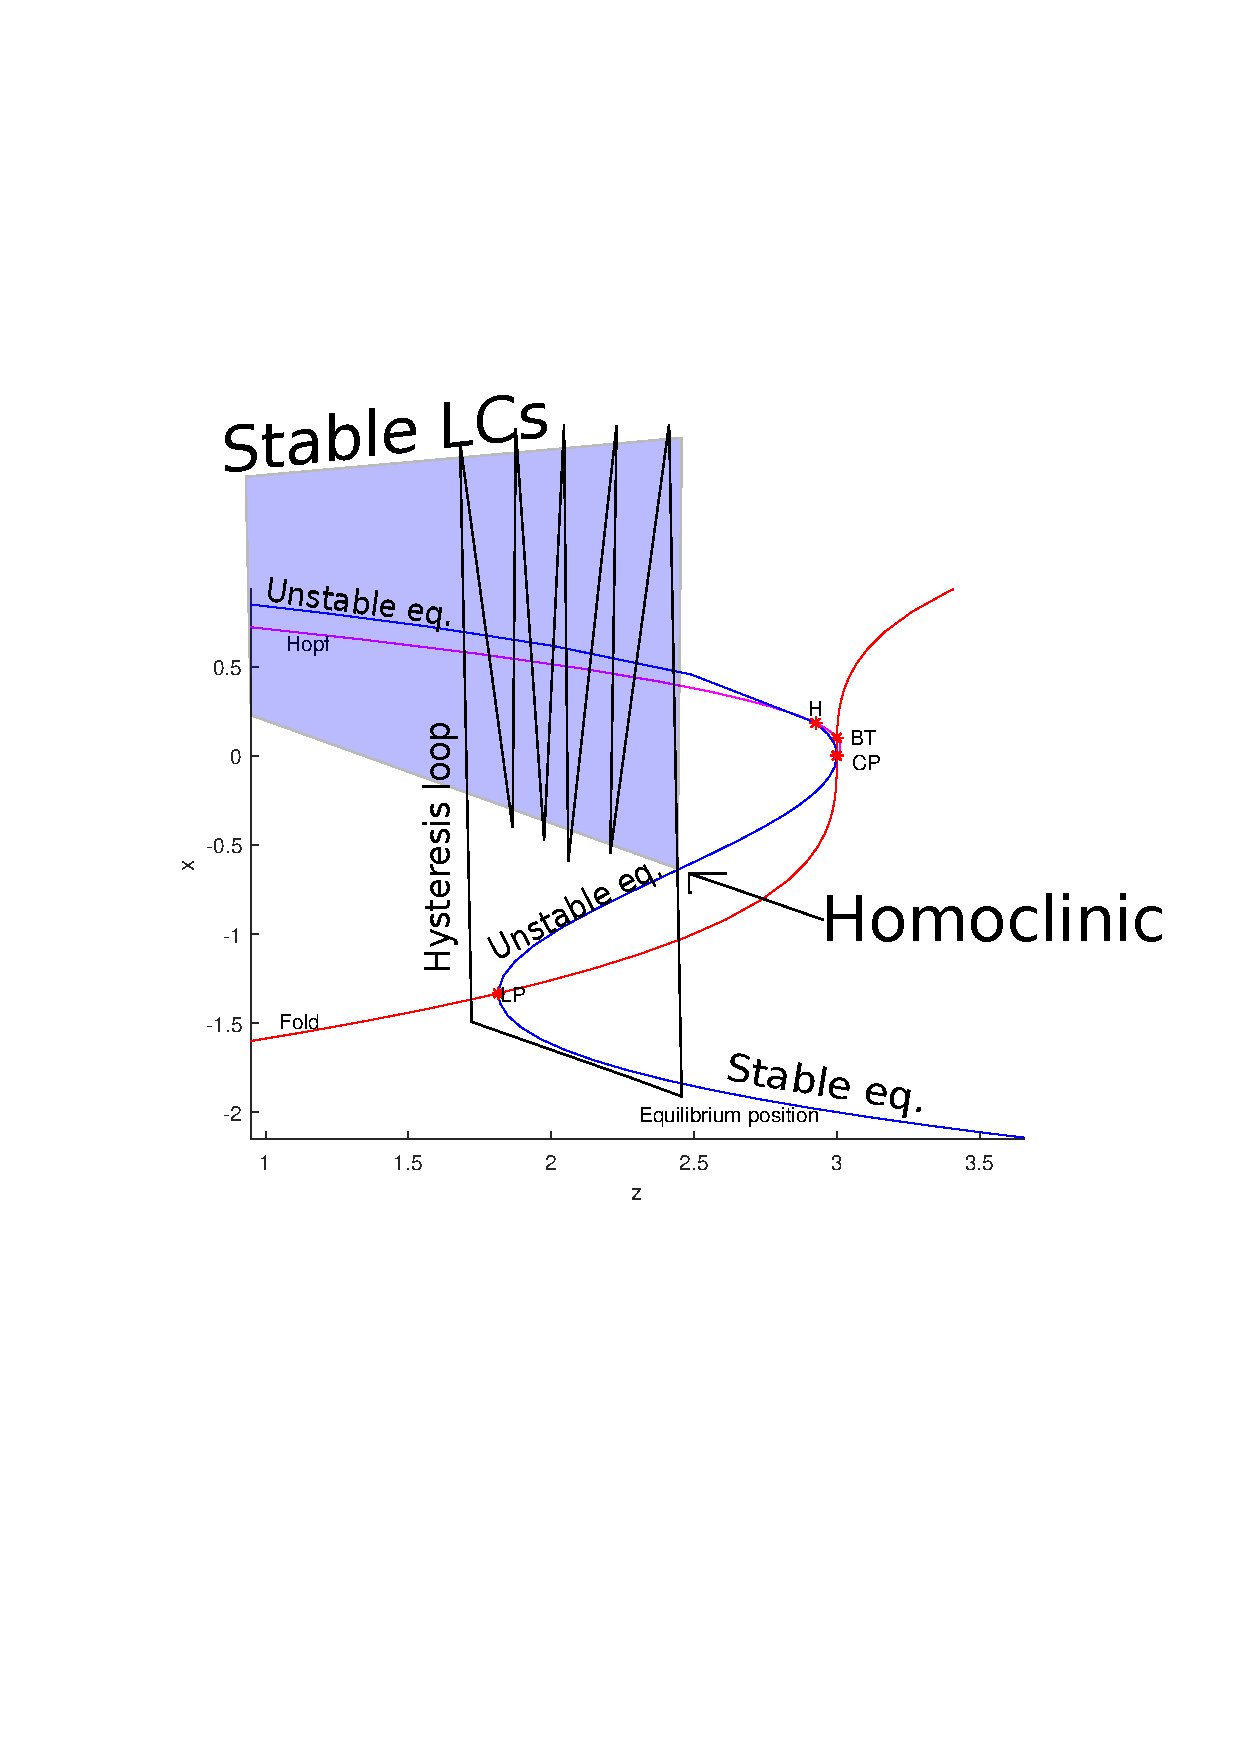
\includegraphics[trim={3cm 9cm 0cm 5cm}, clip,height=.7\textheight]{HRzbBif2 (copy 1).pdf}
\end{center}
\end{column}
\begin{column}{0.4\columnwidth}
\begin{itemize}
\item Homoclinic bifurcations are fundamental to neuron function
\item I can't seem to find them in my Hindmarsh-Rose bifurcation analysis
\end{itemize}
\end{column}
\end{columns}
\end{frame}
\begin{frame}[label={sec:org01ad99d}]{Motivating problem}
\begin{itemize}
\item Homoclinic bifurcations are fundamental to neuron function, so they are a useful thing to understand
\item Bogdanov-Takens points (intersection of Saddle-Node and Hopf bifurcations) necessarily produce a family of homoclinics
\begin{itemize}
\item Krassy's model is an unfolding of a doubly-degenerate Bogdanov-Takens singularity
\item Since it's codim-4, it the parameter space contains three-dimensional subspaces of homoclinic bifurcations
\item The bifurcations are therefore unavoidable!
\end{itemize}
\item CBC can't yet deal with homoclinic bifurcations, making it a particularly interesting area to study
\end{itemize}
\end{frame}

\begin{frame}[label={sec:org2a57769}]{Goals and results}
\begin{itemize}
\item Goal: find and continue homoclinic bifurcations in the HR and Cubic Lienard models
\item Results: \emph{[none]}
\end{itemize}
\end{frame}
\begin{frame}[label={sec:org80b433c}]{The challenges of Homoclinic bifurcations (1)}
The period of a limit cycle diverges to infinity at a homoclinic bifurcation, making numerical integration difficult:
\begin{itemize}
\item Homoclinic trajectories are the solution to a boundary value problem, where the boundaries (start, end state) are a saddle equilibrium
\item The equilibrium is only reached as \(t \to \pm \infty\), meaning our boundaries are not numerically tractable
\item To fix this, we use projective boundary conditions, to truncate the problem onto a finite time domain
\item These require some rather complicated maths
\end{itemize}
\end{frame}

\begin{frame}[label={sec:org98e287d}]{The challenges of Homoclinic bifurcations (2)}
\begin{itemize}[<+->]
\item A homoclinc orbit becomes arbitrarily small at a BT point (small in the Lebesgue measure sense)
\item Homoclinic bifurcations are a \emph{'truly global'} bifurcation - no stability changes occur in any invariant sets
\begin{itemize}
\item Since there's no stability changes, we can only detect these bifurcations by searching for homoclinic trajectories
\end{itemize}
\item But, this becomes impossible near a BT point, since those trajectories become arbitrarily small
\item Looking for homoclinc bifurcations at a BT point therefore becomes a problem of spotting nothing happening, where that nothing happens in an infinitely small region of phase space
\end{itemize}
\end{frame}

\begin{frame}[label={sec:orgaa8dcf4}]{The challenges of Homoclinic bifurcations (3)}
I flicked through a few different papers on the numerical aspects of homoclinic continuation. 
They build on maths that I don't know much about
\begin{itemize}
\item Reduction of the system to the center manifold
\item Homeomorphism onto topological normal forms
\item Everything to do with projective boundary conditions
\item Homotopic shooting methods
\end{itemize}

\emph{Guckenheimer and Holmes (1983)} contains most of the required maths, as well as lots of useful information on bifurcations.
I've added it to my reading list!
\end{frame}


\section{Numerical continuation}
\label{sec:org33208d0}
\begin{frame}[label={sec:org389dab9}]{Week's activities (week 2)}
\begin{itemize}
\item Homoclinic bifurcations are interesting, but would require a large time investment to make any progress
\item Instead, I returned to numerical bifurcation analysis
\begin{itemize}
\item Started learning about PyDSTool
\item Followed online tutorials
\item Managed to generate some bifurcation diagrams
\end{itemize}
\end{itemize}

\end{frame}
\begin{frame}[plain]
\begin{columns}
\begin{column}{0.5\columnwidth}
\begin{center}
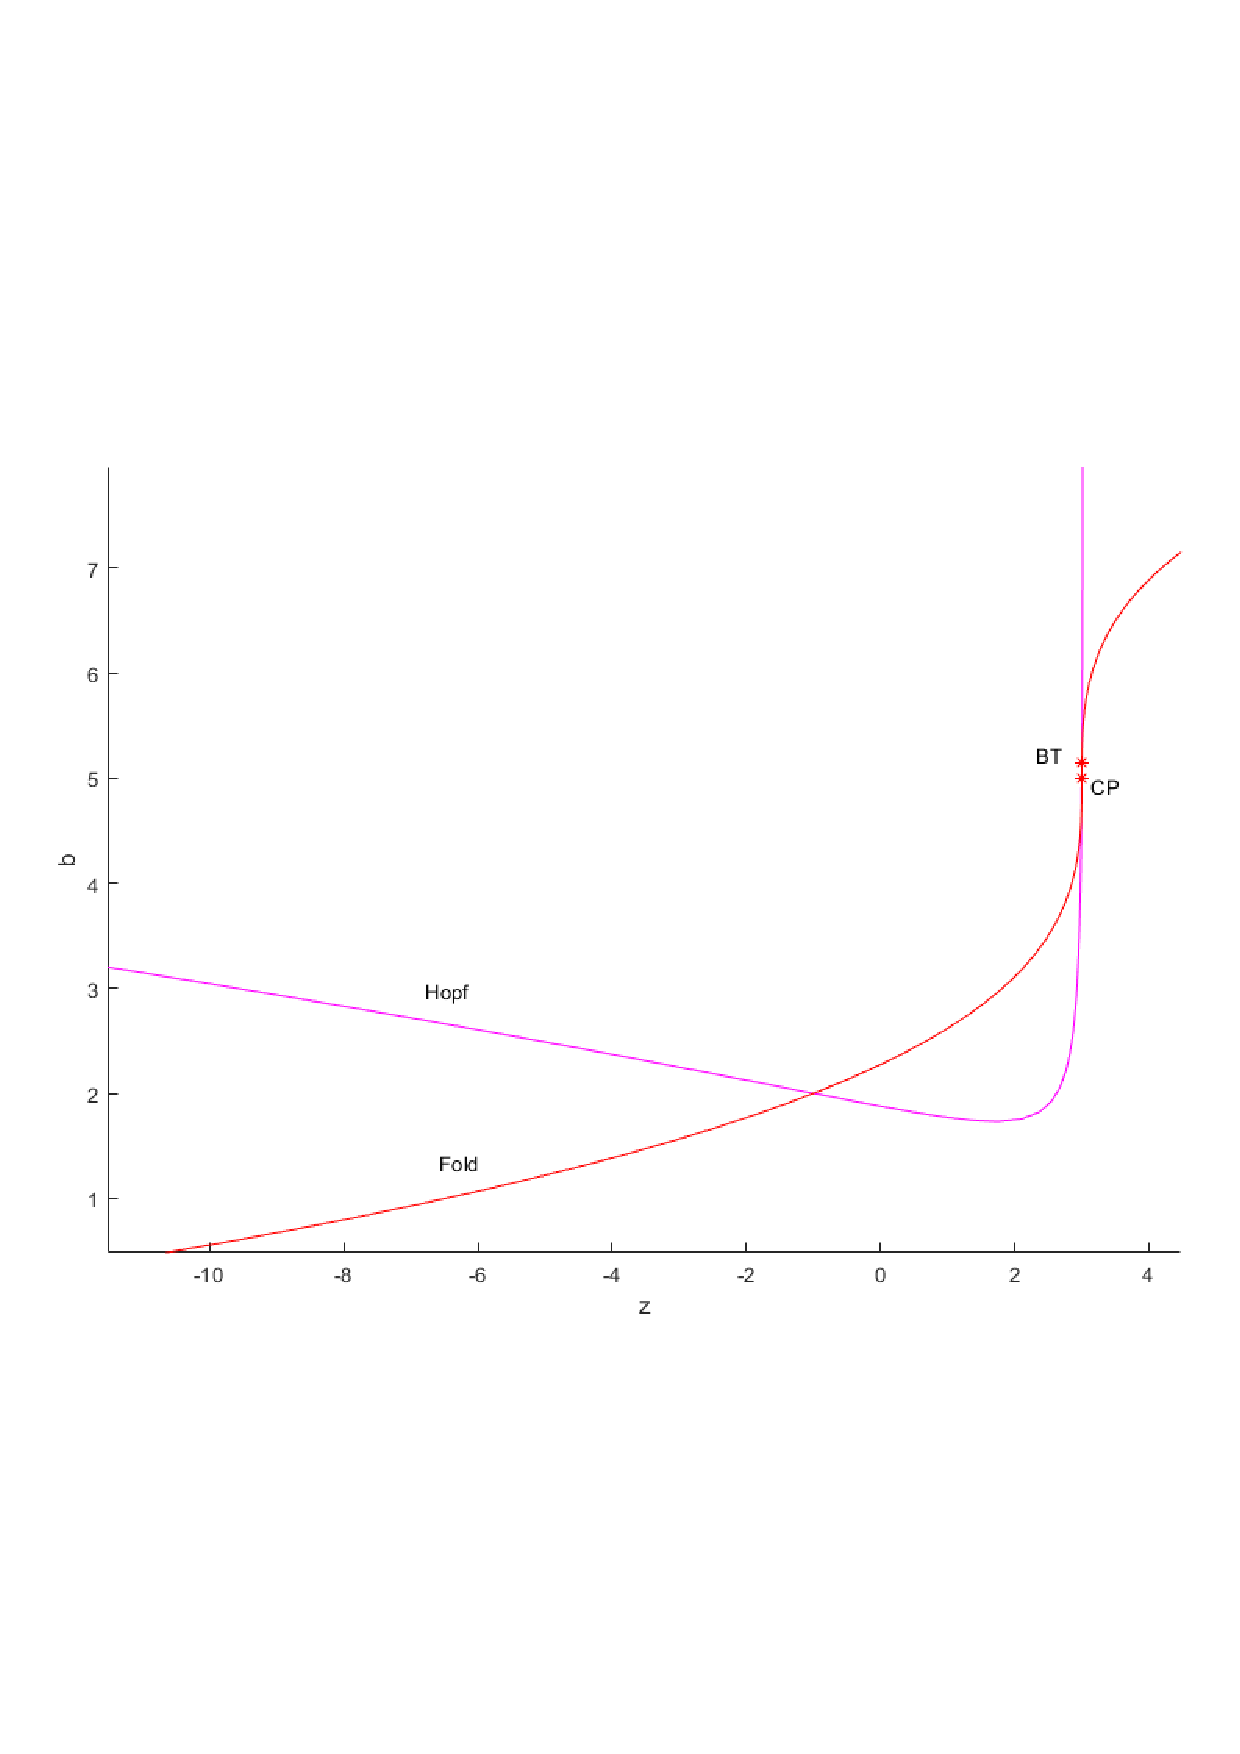
\includegraphics[width=\textwidth]{HRzbBif.pdf}
\end{center}
\end{column}
\begin{column}{0.5\columnwidth}
\begin{center}
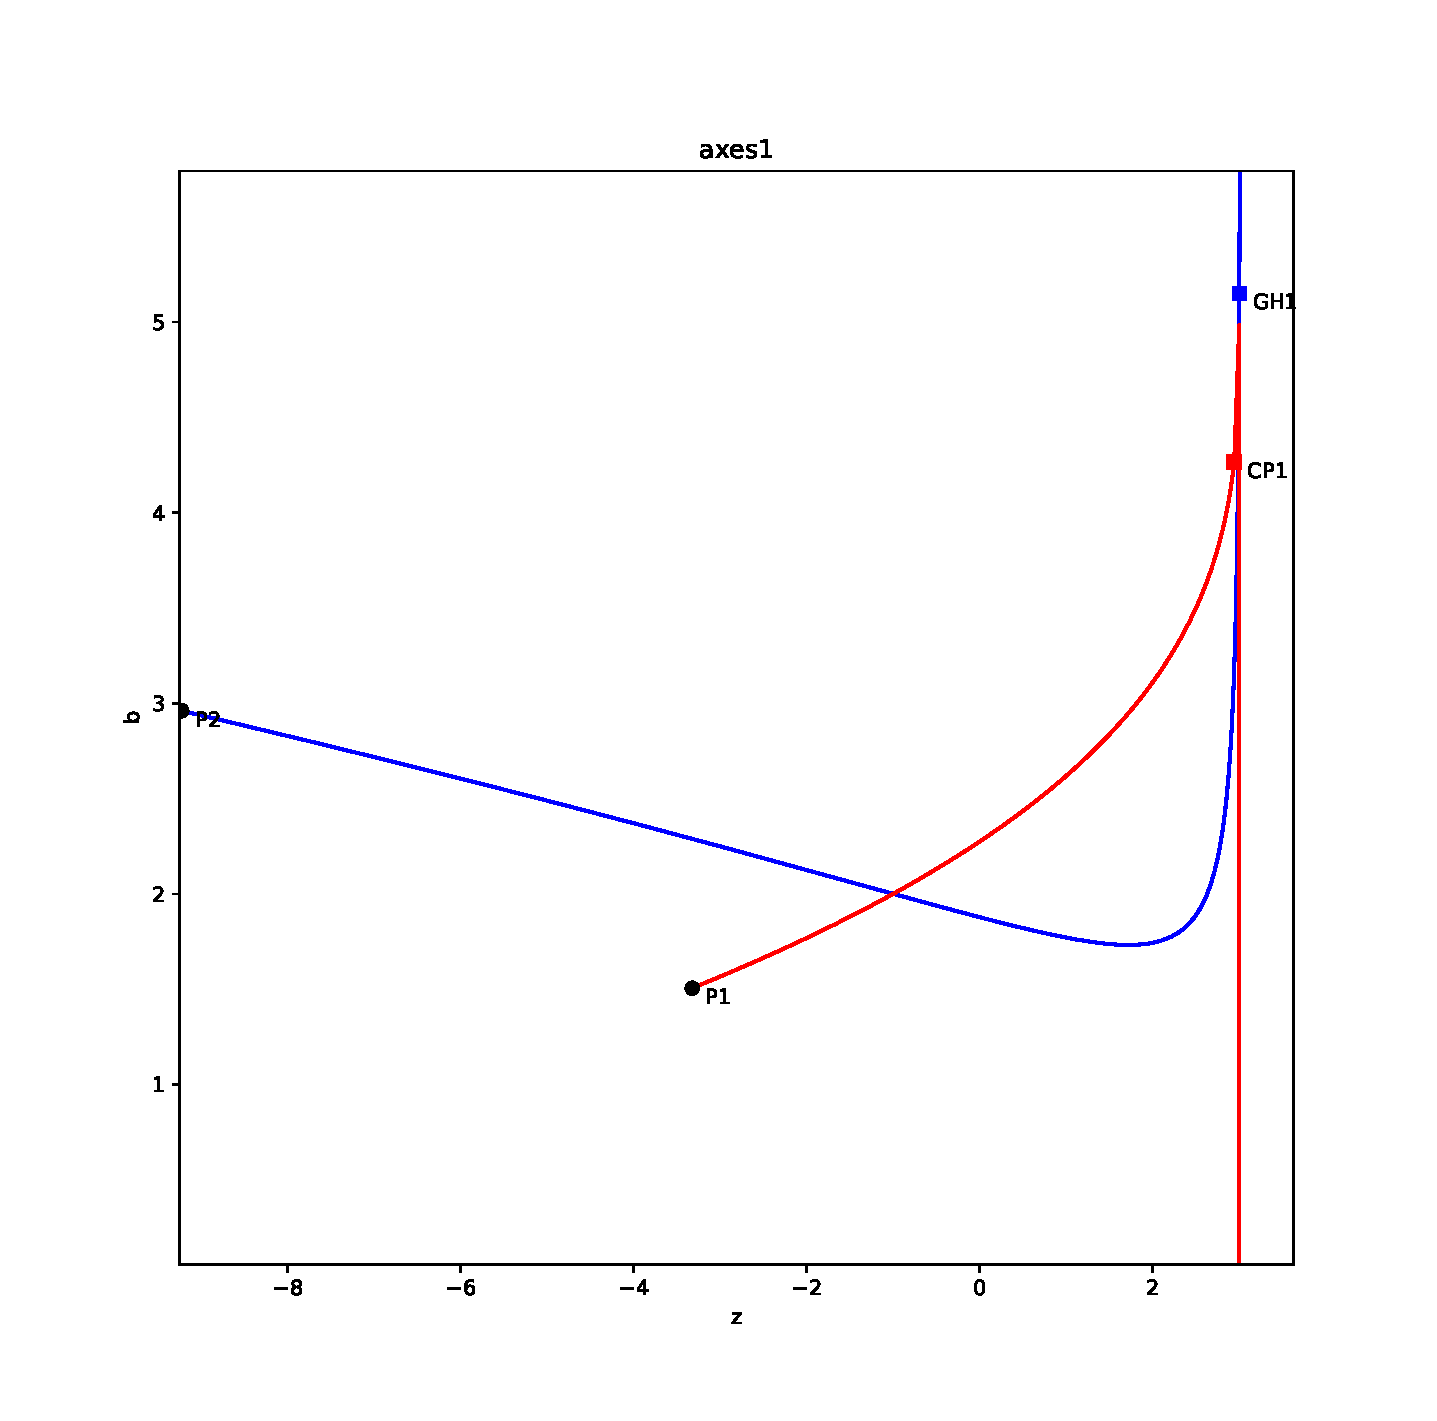
\includegraphics[width=\textwidth]{dstool_2dbif.pdf}
\end{center}
\end{column}
\end{columns}


\end{frame}
\begin{frame}[plain]

\begin{center}
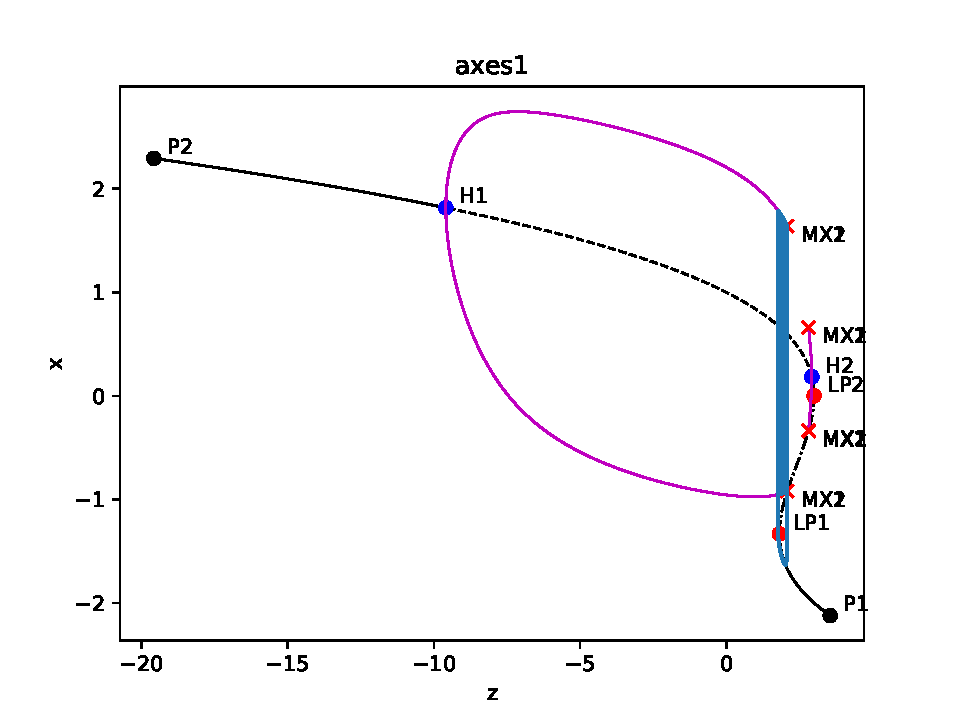
\includegraphics[width=\textwidth]{pydstool3.pdf}
\end{center}


\end{frame}
\begin{frame}[plain]

\begin{center}
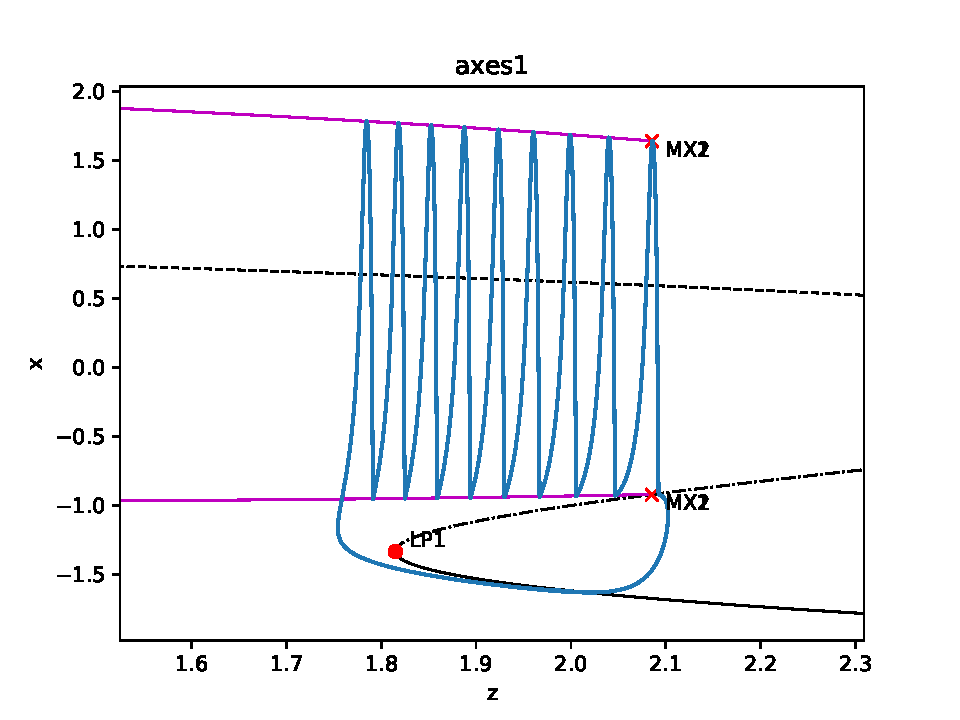
\includegraphics[width=\textwidth]{pydstool4.pdf}
\end{center}


\end{frame}
\begin{frame}[plain]

\begin{center}
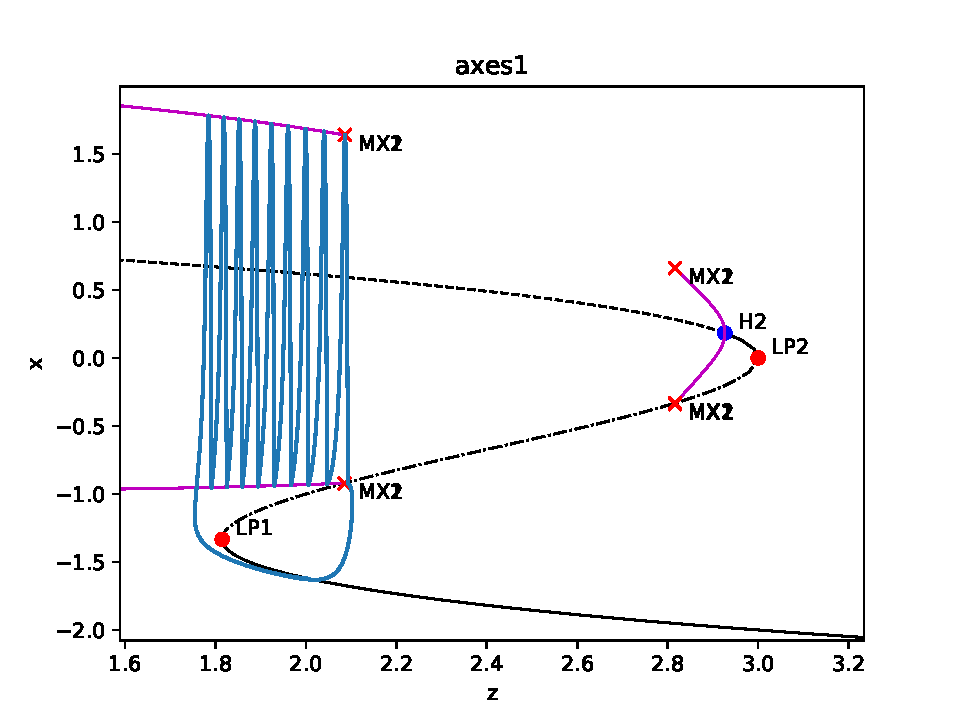
\includegraphics[width=\textwidth]{pydstool2.pdf}
\end{center}
\end{frame}


\section{Next steps}
\label{sec:orgd39a465}
\begin{frame}[label={sec:orgcdb2d33}]{Project ideas}
\begin{enumerate}
\item Find a way of using CBC to track homoclinic bifurcations (challenge: CBC of global bifurcations)
\begin{itemize}
\item Use the simplest possible system and the simplest possible controller
\item Use that knowledge to add homoclinic bifurcation analysis into PyDSTool, if it won't take too long to do so? Might be paper-worthy in itself?
\end{itemize}
\item Design a controller that'll work on neuron models; adapt the CBC approach to use Krassy's model and the new controller (challenge: discretising spiking signals, controlling neurons)
\begin{itemize}
\item Use that for an in-silico neuron CBC simulation
\item See how things change when noise gets introduced
\end{itemize}
\item Use the newly developed CBC approach on a real live neuron (challenge: experiments)
\end{enumerate}
\end{frame}
\begin{frame}[label={sec:orgadc513a}]{Next steps}
\begin{itemize}
\item Keep learning numerical continuation tools (next steps: CoCo, MATCONT CL)
\item Start writing some notes about the ones I've used so far
\begin{itemize}
\item QUESTION: what sort of things would be useful to discuss in the paper?
\end{itemize}
\item Mix things up with some \emph{Guckenheimer and Holmes}, when I get tired
\end{itemize}
\end{frame}
\end{document}
